\documentclass{article}
% main document, called main.tex
\usepackage{tikz}
\usetikzlibrary{external}

\usepackage{color,soul}
\definecolor{light-gray}{gray}{0.95} 
\DeclareRobustCommand{\hlcyan}[1]{{\sethlcolor{cyan}\hl{#1}}}
\DeclareRobustCommand{\hlgreen}[1]{{\sethlcolor{green}\hl{#1}}}

\colorlet{orangegreen}{green!10!orange!90!}
\definecolor{darkgreen}{rgb}{0, 0.5, 0} 

\usetikzlibrary{positioning}
\usetikzlibrary{calc}
\usetikzlibrary{shapes.geometric, arrows, arrows.meta}
\usepackage{varwidth}% http://ctan.org/pkg/varwidth
\usetikzlibrary{shadows,trees, mindmap}
\usetikzlibrary{matrix}
\usetikzlibrary{fit}

\tikzexternalize % activate!
\begin{document}
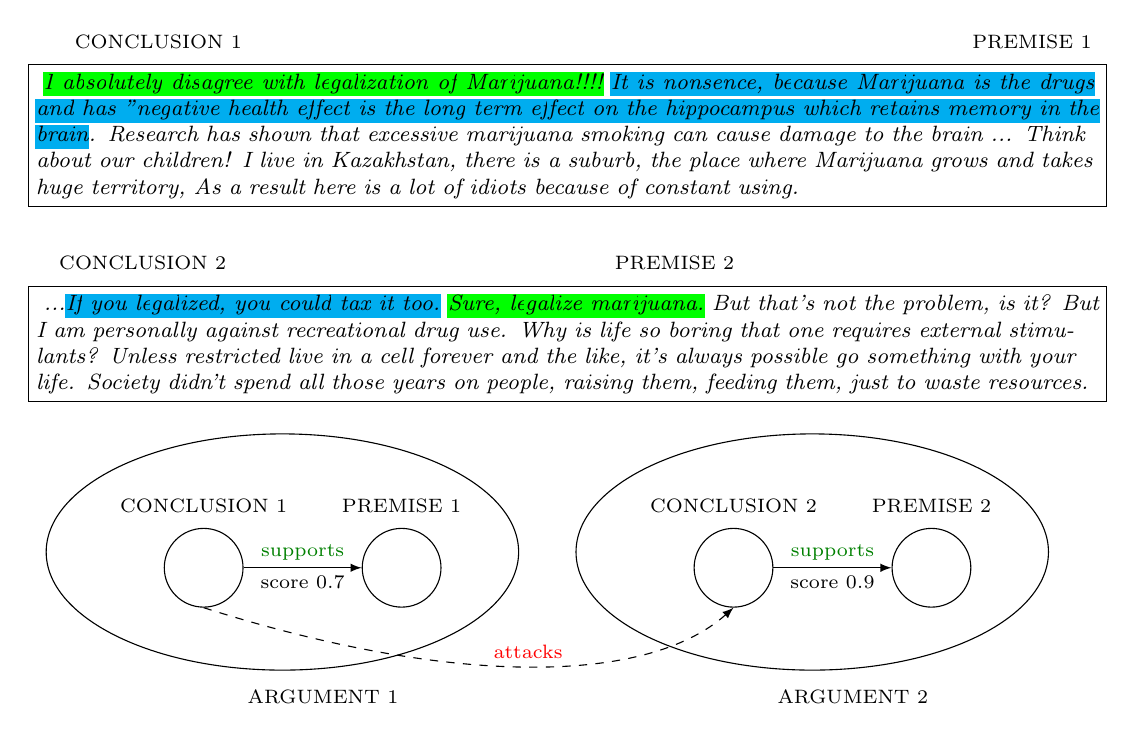
\begin{tikzpicture}
[
textbox/.style={rectangle, draw, text width=13.5cm, align=left, 
	},
arg/.style={circle, draw, minimum size=1cm}
]
	\footnotesize{
	\node (text1) [textbox] {
\emph{
	\hlgreen{I absolutely disagree with legalization of Marijuana!!!!}
	\hlcyan{It is nonsence,
	because Marijuana is the drugs and has "negative health effect is the
	long term effect on the hippocampus which retains memory in the brain}.
Research has shown that excessive marijuana smoking can cause damage to
the brain ...  Think about our children! I live in Kazakhstan, there is
a suburb, the place where Marijuana grows and takes huge territory, As
a result here is a lot of idiots because of constant using.
}
};
\node (text2) [textbox, below=1 cm of text1] {
\emph{
	...\hlcyan{If you legalized, you could tax it too.} \hlgreen{Sure,
	legalize marijuana.} But that's not the problem, is
	it? But I am personally against recreational drug use.
	Why is life so boring that one requires external stimulants?
	Unless restricted live in a cell forever and the like, it's always
	possible go something with your life. Society didn't spend all
	those years on people, raising them, feeding them, just to waste
	resources.
}
};
}
	\scriptsize{
	\node (conclusion1) [above right=0.1cm and 0.5cm of text1.north west] {CONCLUSION 1};
	\node (premise1) [above left=0.1cm and 0.1cm of text1.north east] {PREMISE 1};
	\node (conclusion2) [above right=0.1cm and 0.3cm of text2.north west] {CONCLUSION 2};
	\node (premise2) [above right=0.1cm and 0.5cm of text2.north] {PREMISE 2};
	}

	\node (invisible) [below=2cm of text2.south] {};
	\node (support1) [arg, left=1.5cm of invisible] {};
	\node (claim2) [arg, right=1.5cm of invisible] {};
	\node (claim1) [arg, left=1.5cm of support1] {};
	\node (support2) [arg, right=1.5cm of claim2] {};

	\scriptsize{
	\node (conclusion1) [above=0.1cm of claim1] {CONCLUSION 1};
	\node (premise1) [above=0.1cm of support1] {PREMISE 1};
	\node (conclusion2) [above=0.1cm of claim2] {CONCLUSION 2};
	\node (premise2) [above=0.1cm of support2] {PREMISE 2};

	\draw[-latex]  (claim1) -- (support1) 
	node [above, midway] {\textcolor{darkgreen}{supports}} node [below, midway] {score $0.7$} ; 

	\draw[-latex]  (claim2) -- (support2) 
	node [above, midway] {\textcolor{darkgreen}{supports}} node [below, midway] {score $0.9$} ; 

	\draw[-latex, dashed] (claim1.south) .. 
	controls ($(invisible) + (-1.5cm, -1.5cm)$ ) and ($(invisible) + (1cm, -1.5cm)$ )
	.. node[above, sloped] {\textcolor{red}{attacks}} (claim2.south);
	

	\draw ($(claim1) + (1cm, 0.2cm)$ ) ellipse (3 cm and 1.5cm);
	\draw ($(claim2) + (1cm, 0.2cm)$ ) ellipse (3 cm and 1.5cm);

	\node (arg1) [below right=1.1cm and 0.1cm of claim1] {ARGUMENT 1};
	\node (arg2) [below right=1.1cm and 0.1cm of claim2] {ARGUMENT 2};
	}
	% connect them

\end{tikzpicture}
\end{document}
